\chapter{Discussion}\label{chp6:discussion}

In this chapter we will discuss the viability of the low frequency acoustic emanations, and how current guidelines for shielding information systems are helping against this threat.
We will also look at the cost involved in building a setup able to process these emanations, and the implications of this.
Lastly we will look at use cases where the analysis of these emanations can be useful.

\section{Viability of Extracted Information}
We have not obtained a basis for drawing a conclusion as to whereas the emanations as presented in the previous chapters are in fact caused by the \gls{CPU}.
However, we have tried to capture the effect at different positions on our Lenovo T60p laptop. 
For this specific computer we experienced that it is far easier to find the patterns we are looking for in the resulting power spectra when the recordings are done right above the \gls{CPU}.
We also found that slight disposition of the microphone of a couple of centimeters, while still hovering the \gls{CPU} cooling block, notably impact the signal strength.


\section{Significance of Results}

We did not do any experiments to verify whether the captured signatures are in fact acoustic, or if they are caused by electromagnetic emanations.
However, we rely on the work by Genkin et al., who discuss this question in detail~\cite[Section 3.3]{DBLP:journals/iacr/GenkinST13}.
Using the acoustic side channel, we are able to distinguish between the \texttt{MEM} operation and the other microinstruction loops.
~\autoref{fig:T60p-knowles-micro-ips-0} is a display of how this is difference is visible for many frequencies in the frequency range.
The results given in~\cite[Fig.~2]{DBLP:conf/crypto/GenkinST14} suggest that it is possible to observe a difference, even between the different microinstructions \texttt{ADD}, \texttt{MUL} and \texttt{NOP}. 
However, the most visible difference they present is in a frequency range much higher than the hard limit imposed on us by the sampling rate of our setup.
Result presented in \autoref{chp5:results} are therefore inconclusive when it comes to distinguishing between the \texttt{NOP}, \texttt{MUL} and \texttt{ADD} operations.


We have conducted experiments using different configurations of hardware and observe big variations in acoustic fingerprints for the different computers, as seen in~\autoref{fig:comparison_micorinstructions}.
An interesting side note is how the acoustic emanations of the Lenovo T60p laptop is changing depending on if the computer is running on battery power (\autoref{fig:comparison_T60p-ekkofritt-bk-micro-ips-3}) or with a power adapter (\autoref{fig:comparison_T60p-ekkofritt-bk-micro-eps-1}).
We believe that the noise introduced by the \gls{AC} power adapter is not emanating from the power adapter itself, as we have experimented with the positioning of the adapter, without seeing any impact on the resulting acoustic signatures.

\begin{figure}[ht]
    \centering
    \begin{subfigure}{0.32\textwidth}
        \centering
        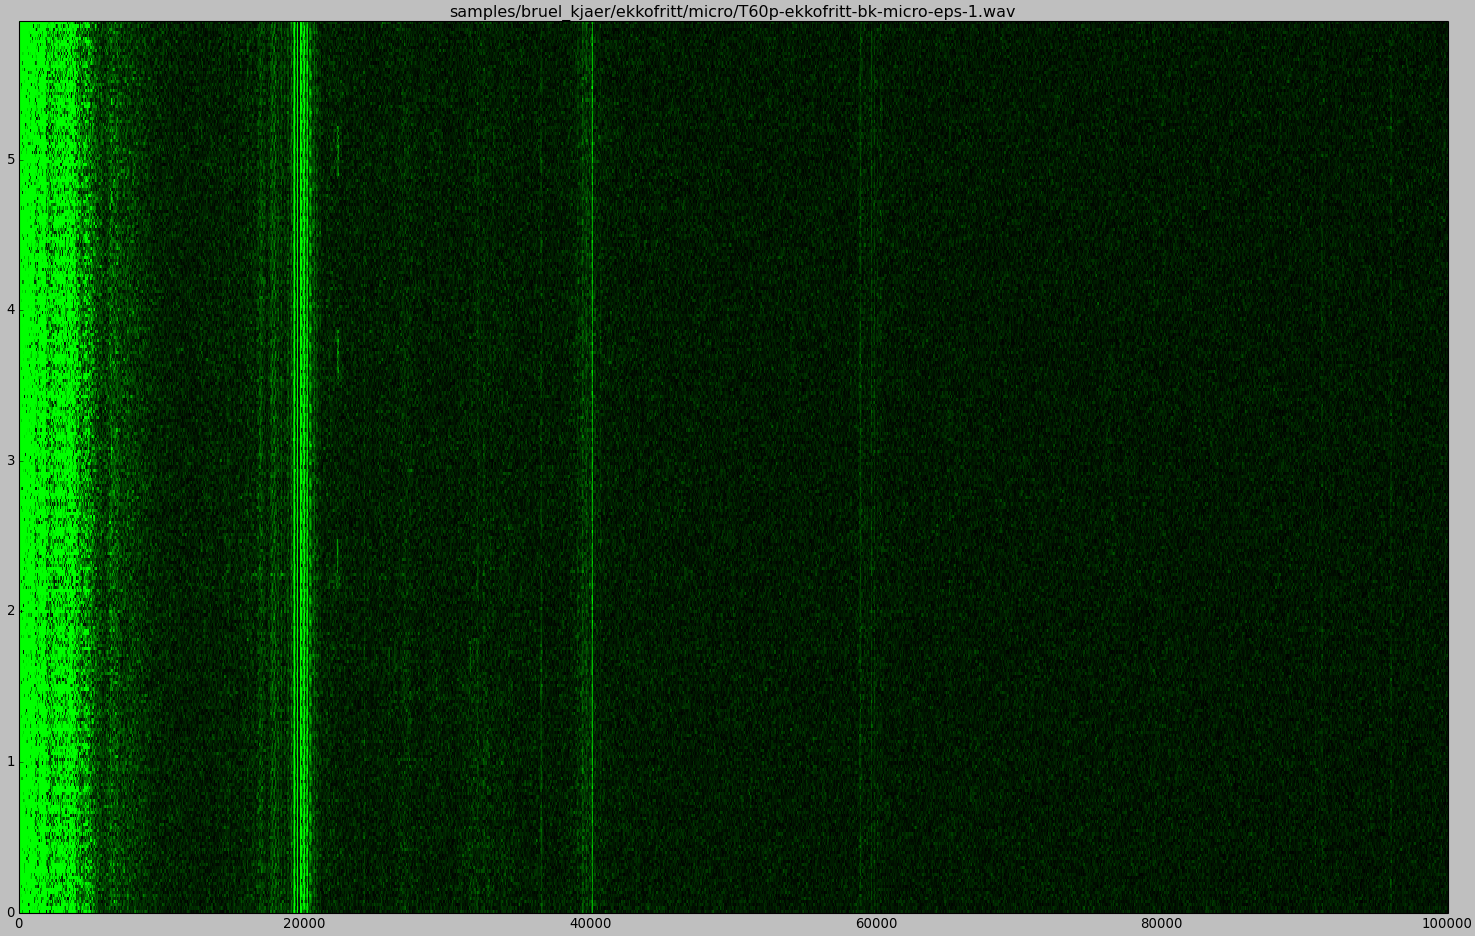
\includegraphics[width=1\linewidth]{T60p-ekkofritt-bk-micro-eps-1.png}
        \caption{Lenovo T60p}
        \label{fig:comparison_T60p-ekkofritt-bk-micro-eps-1}
    \end{subfigure}
    \begin{subfigure}{0.32\textwidth}
        \centering
        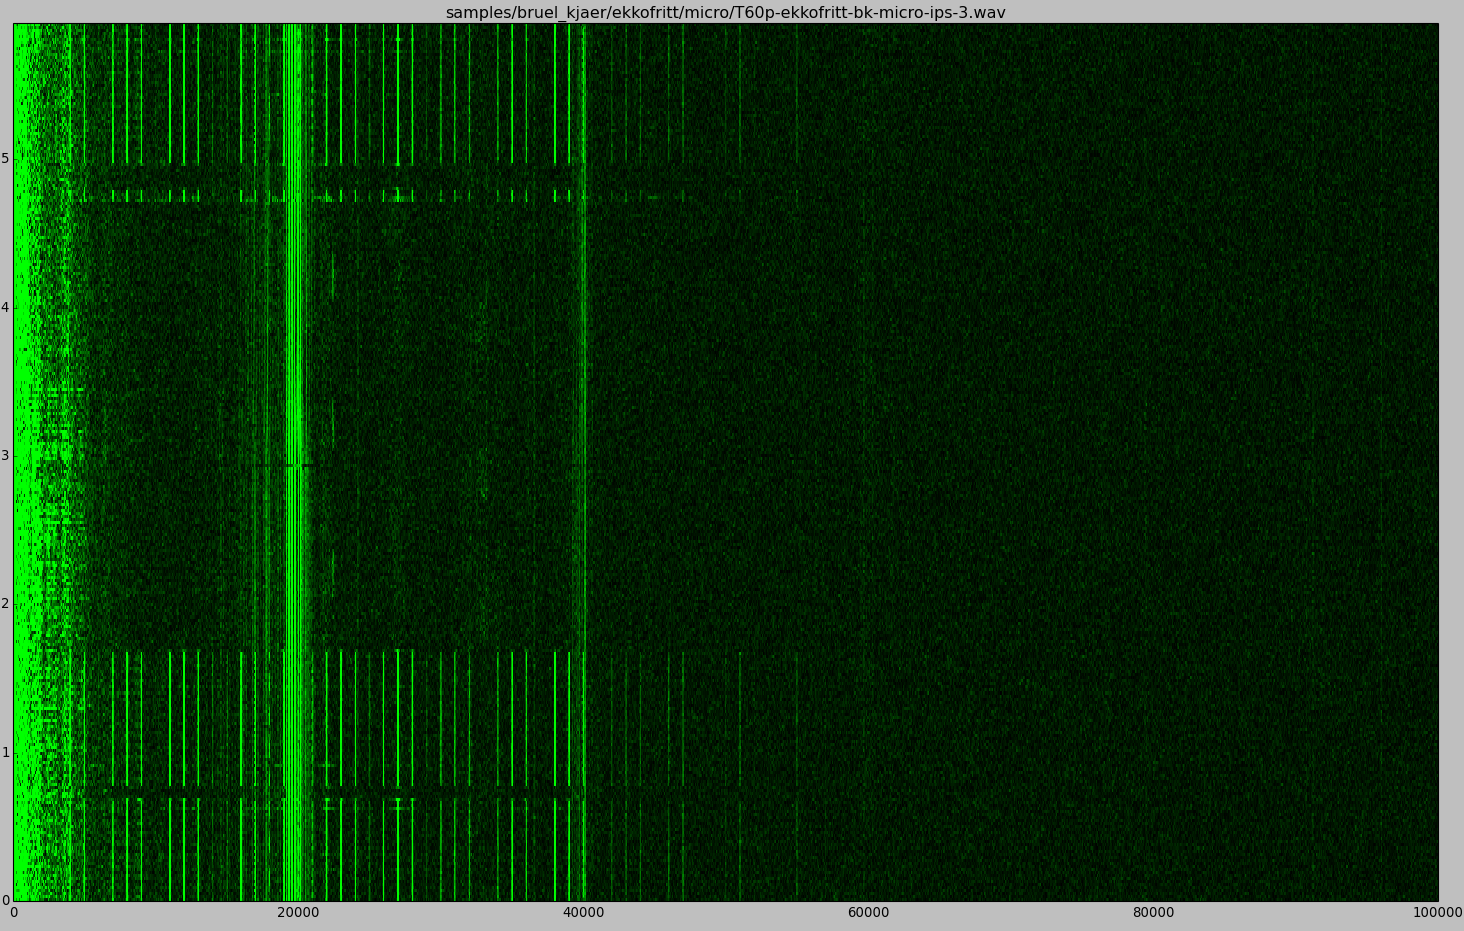
\includegraphics[width=1\linewidth]{T60p-ekkofritt-bk-micro-ips-3.png}
        \caption{Lenovo T60p}
        \label{fig:comparison_T60p-ekkofritt-bk-micro-ips-3}
    \end{subfigure}
    \begin{subfigure}{0.32\textwidth}
        \centering
        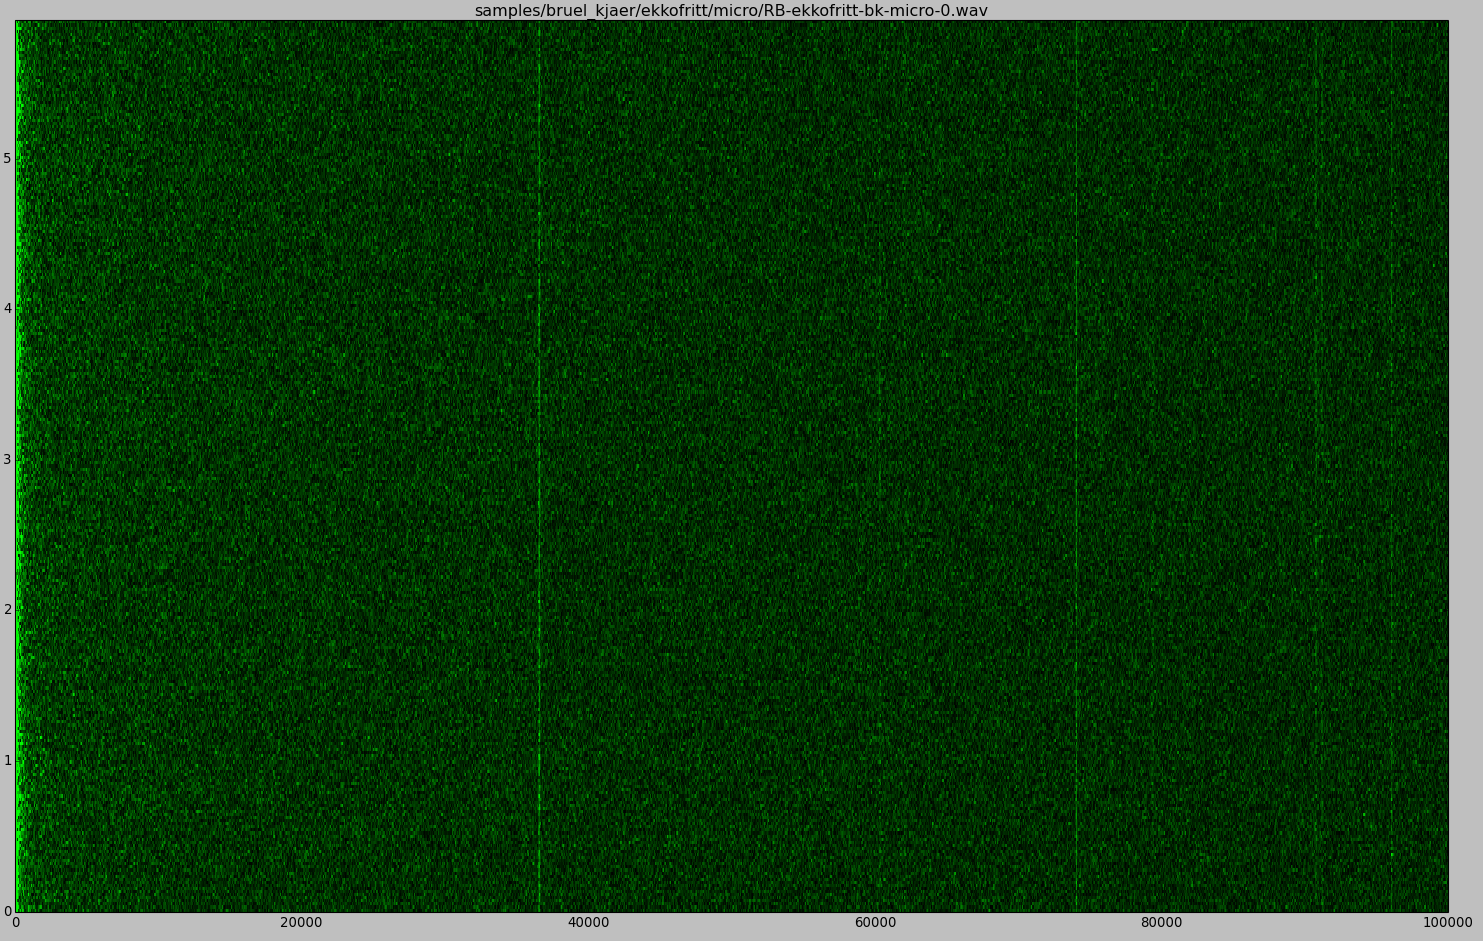
\includegraphics[width=1\linewidth]{RB-ekkofritt-bk-micro-0.png}
        \caption{Raspberry PI}
        \label{fig:comparison_RB-ekkofritt-bk-micro-0}
    \end{subfigure}
    \begin{subfigure}{0.32\textwidth}
        \centering
        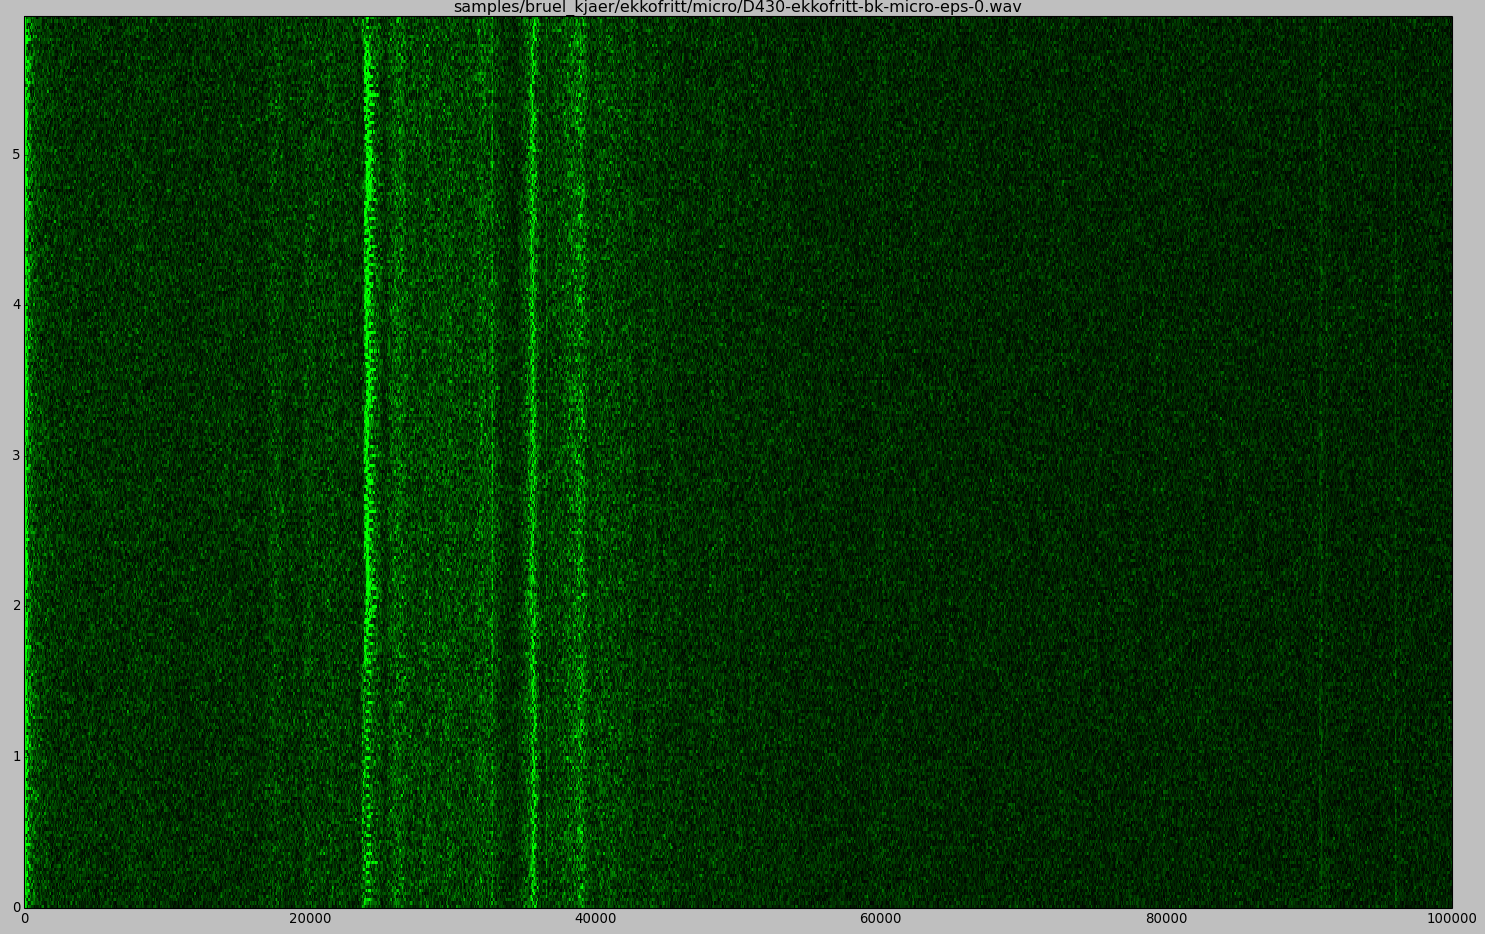
\includegraphics[width=1\linewidth]{D430-ekkofritt-bk-micro-eps-0.png}
        \caption{Dell 430}
        \label{fig:comparison_D430-ekkofritt-bk-micro-eps-0}
    \end{subfigure}
    \begin{subfigure}{0.32\textwidth}
        \centering
        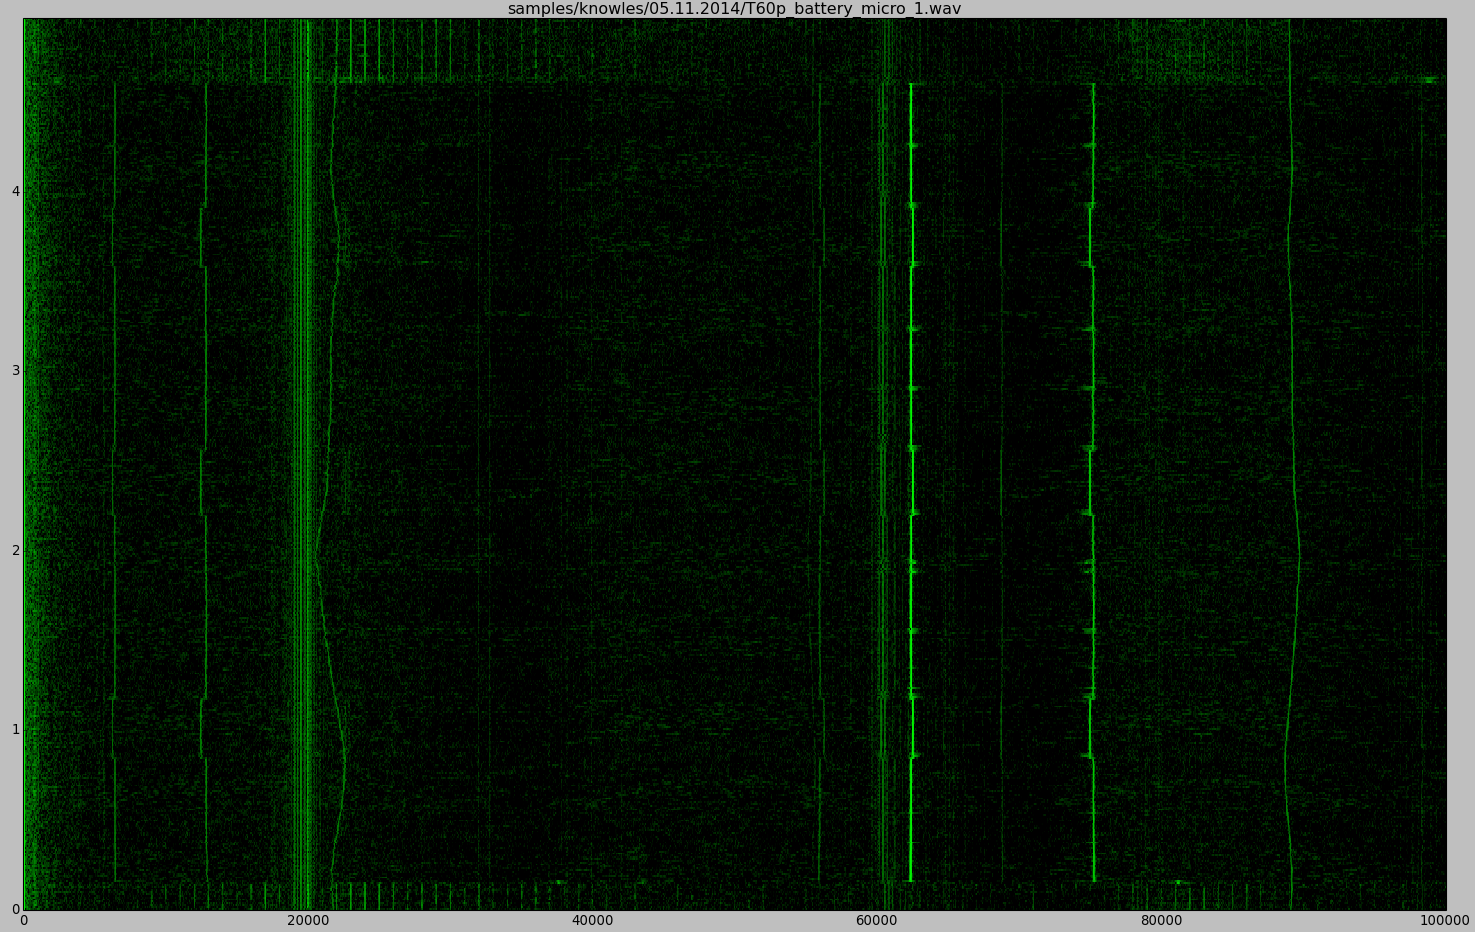
\includegraphics[width=1\linewidth]{T60p-knowles-micro-ips-0.png}
        \caption{Lenovo T60p}
        \label{fig:comparison_T60p-knowles-micro-ips-0}
    \end{subfigure}
    \begin{subfigure}{0.32\textwidth}
        \centering
        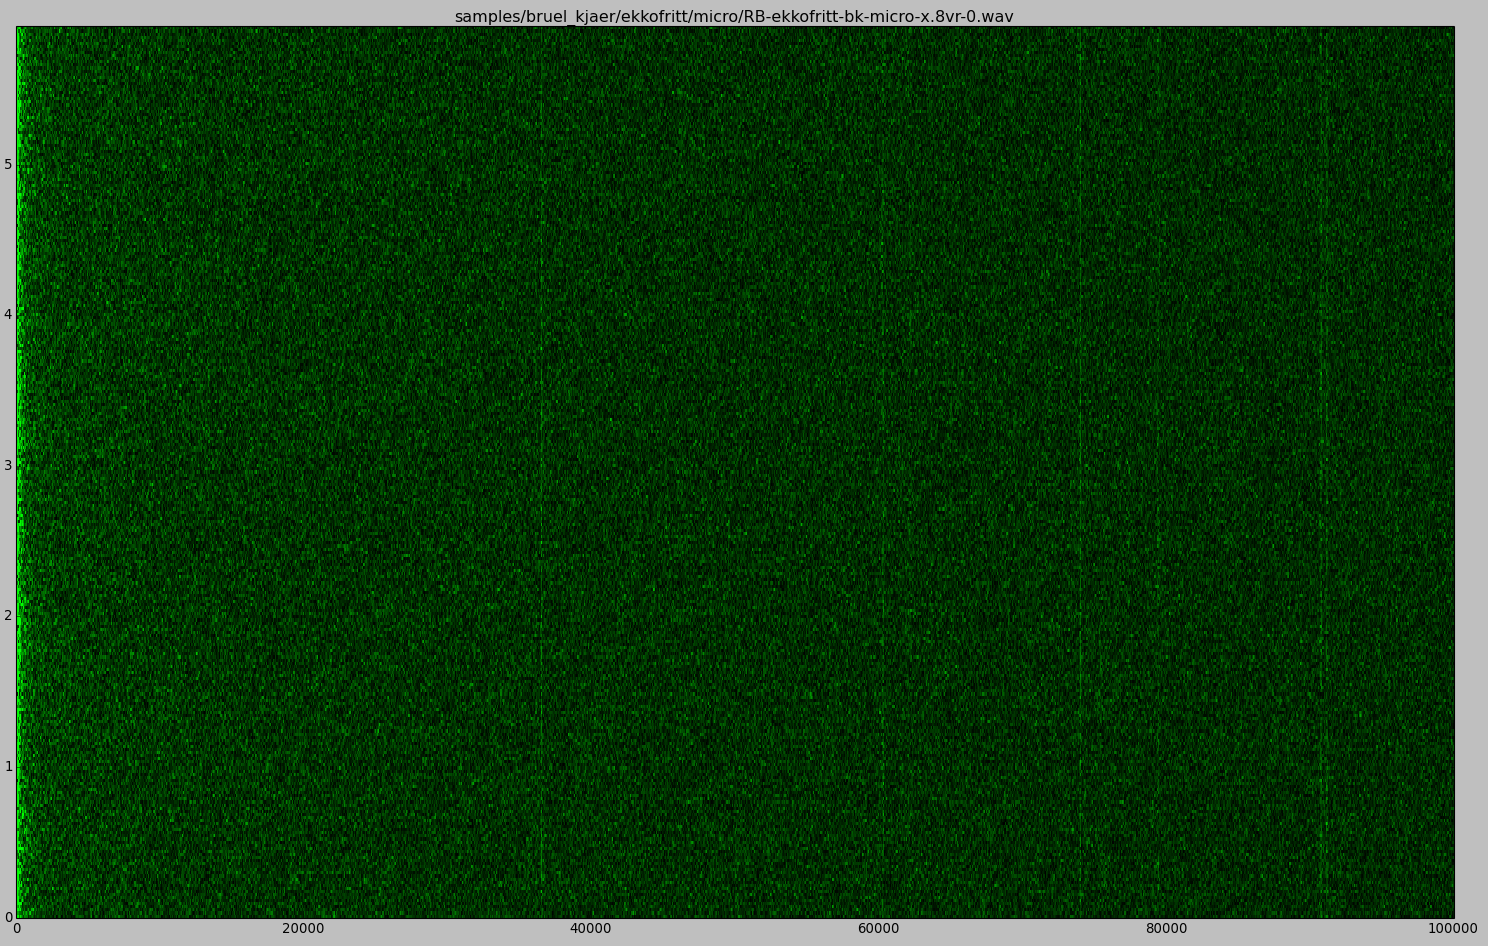
\includegraphics[width=1\linewidth]{RB-ekkofritt-bk-micro-x-8vr-0.png}
        \caption{Raspberry PI}
        \label{fig:comparison_RB-ekkofritt-bk-micro-x-8vr-0}
    \end{subfigure}
    \caption{ Acoustic signatures when running the CPU operations experiment on following devices:
    (a) T60p with \gls{AC} power adopter (lab-grade setup).
    (b) T60p on battery power (lab-grade setup).
    (c) Raspberry PI recording the CPU (lab-grade setup).
    (d) D430 on battery power (lab-grade setup).
    (e) T60p on battery power (portable setup).
    (f) Raspberry PI recording the CPU (lab-grade setup).}
    \label{fig:comparison_micorinstructions}
\end{figure}

\section{Analysis Beyond Extremes}
In our experiments, we were able to distinguish between different extremes in \gls{CPU} activity based visual representation of the acoustic leakage. 
We do not use any mathematical models, but rely on empirical analysis of the power spectra. 
This is a limiting factor in the sense that we are only able to draw conclusions based on clear patterns in the resulting data that are visible to the human eye, when presented in the way done here and by Genkin et al.
None of the experiments we performed included real-time analysis of the leakage, hence we were limited to look for patterns resulting from static programs being executed to be able to relate the information captured to the time domain in our offline analysis.
Real-time analysis, together with mathematical models for correlation, would allow a more statistical approach to distinguishing between distinct fingerprints, and could allow for attacks along the line of what is proposed in~\cite{DBLP:conf/crypto/KocherJJ99}, only using acoustic emanations rather than power traces for analysis.


\section{ARM Processors and Possible Attack Vectors}
We chose to conduct experiments on a Lenovo laptop computer similar to what is used by Genkin et al., and also on an even older Dell laptop, as it was suggested that older processors had more explicit acoustic fingerprints.
In addition, we conducted the same experiments for a Raspberry Pi, which is equipped with an ARM \gls{CPU}.

A motivation for looking at ARM processors is that a lot of electronic equipment today is running on the ARM architecture.
The potential of analyzing network traffic by looking at routers is just one of several interesting approaches to exploit the potential of low frequency acoustic emanations.
Unfortunately, we found it much harder to distinguish between operations on the Raspberry Pi, than for the laptops running on x86/x64 Intel processors.
It is still worth noting that the findings of Genkin et al. suggest that distinguishing between different RSA keys used for decryption can be done using this side channel; in the case of a router, this means that the approach could be a viable way to analyze ongoing IPSec sessions, where the router performs encryption or decryption, without being connected to the network at all.


\section{Possible Attack Scenarios}\label{chp6:sec:attack_scenarios}

Our portable setup (\autoref{chp3:sec:knowles_configuration}) could be made even smaller and mounted with a small transmitter. 
This makes the setup mountable on stationary computers, where it could be used for eavesdropping. 

Manufacturers with malicious intentions can mount a small ultrasound microphone on a selection of devices from a batch, which in many cases will not be discovered.

Genkin et al. introduces some possible attack scenarios that could exploit the acoustic emanations in~\cite[Section 1.2 and Appendix B]{DBLP:journals/iacr/GenkinST13}, like an acoustic attack app and self-eavesdropping.

\section{Countermeasures}\label{chp6:sec:countermeasures}

In the guidance paper about protection against eavesdropping published by the \gls{NSM}, it is recommended that one should follow the TEMPEST guidance when installing an information system~\cite[Section 9.8, page 7]{url:NSM/avlytting}.
However, the shielding requirement for a TEMPEST certified equipment is made with respect to electromagnetic signals.
Thus TEMPEST requirements for shielding (e.g. a Faraday cage) might not protect against acoustic emanations. 

The Red/Black Engineering-Installation Guidelines~\cite[Section 30.1, page 91]{url:Red/Black/Engineering} created by the \gls{DoD}, states that unauthorized (BLACK) and authorized (RED) equipment should at least be separated with 3 feet (roughly 0.9 m).
Other electronic devices such as mobile phones and personal laptops should not be permitted to areas where RED equipment is installed. 
Genkin et al. were able to recover a 4096-bit RSA key from a distance of 10 meters, thus an air gap of 0.9 meters will not suffice in canceling the acoustic side-channel itself.

The frequency signatures presented in this paper are leaking information in the audible range of the human ear.
Yet, our target computers are relatively old laptops, and our results add to the suspicion of Genkin et al. that the quality of information in the side-channel seems correlated to the computer's age.
Hence, it might be harder to extract information using the acoustic side channel on newer computers.
We have also added to this theory that ARM processors arguably are not viable targets, as our results show no visible correlation between CPU operations and acoustic signature.
